\section{Introduction}
The stationary heat equation is considered for a two-dimensional plate,
\begin{gather}
    -\nabla\cdot\left(k\nabla T\right)=0.
\end{gather}\label{eq:heat}The plate defines the domain $\Omega\prime= \Omega_A\prime\cup\Omega_B\prime \subset \mathbb{R}^2$. $\Omega_A$ has width $b$ and height $h$ with heat conductivity $k_A$. In the center of the plate a rectangular area is embedded with width $b_0$, height $h_0$ and heat conductivity $k_B$. The domain, has boundary $\Gamma=\Gamma_1\prime\cup\Gamma_2\prime\cup\Gamma_3\prime\cup\Gamma_4\prime$. See Figure~\ref{fig:domain}. 
\begin{Figure}
 \centerfloat
 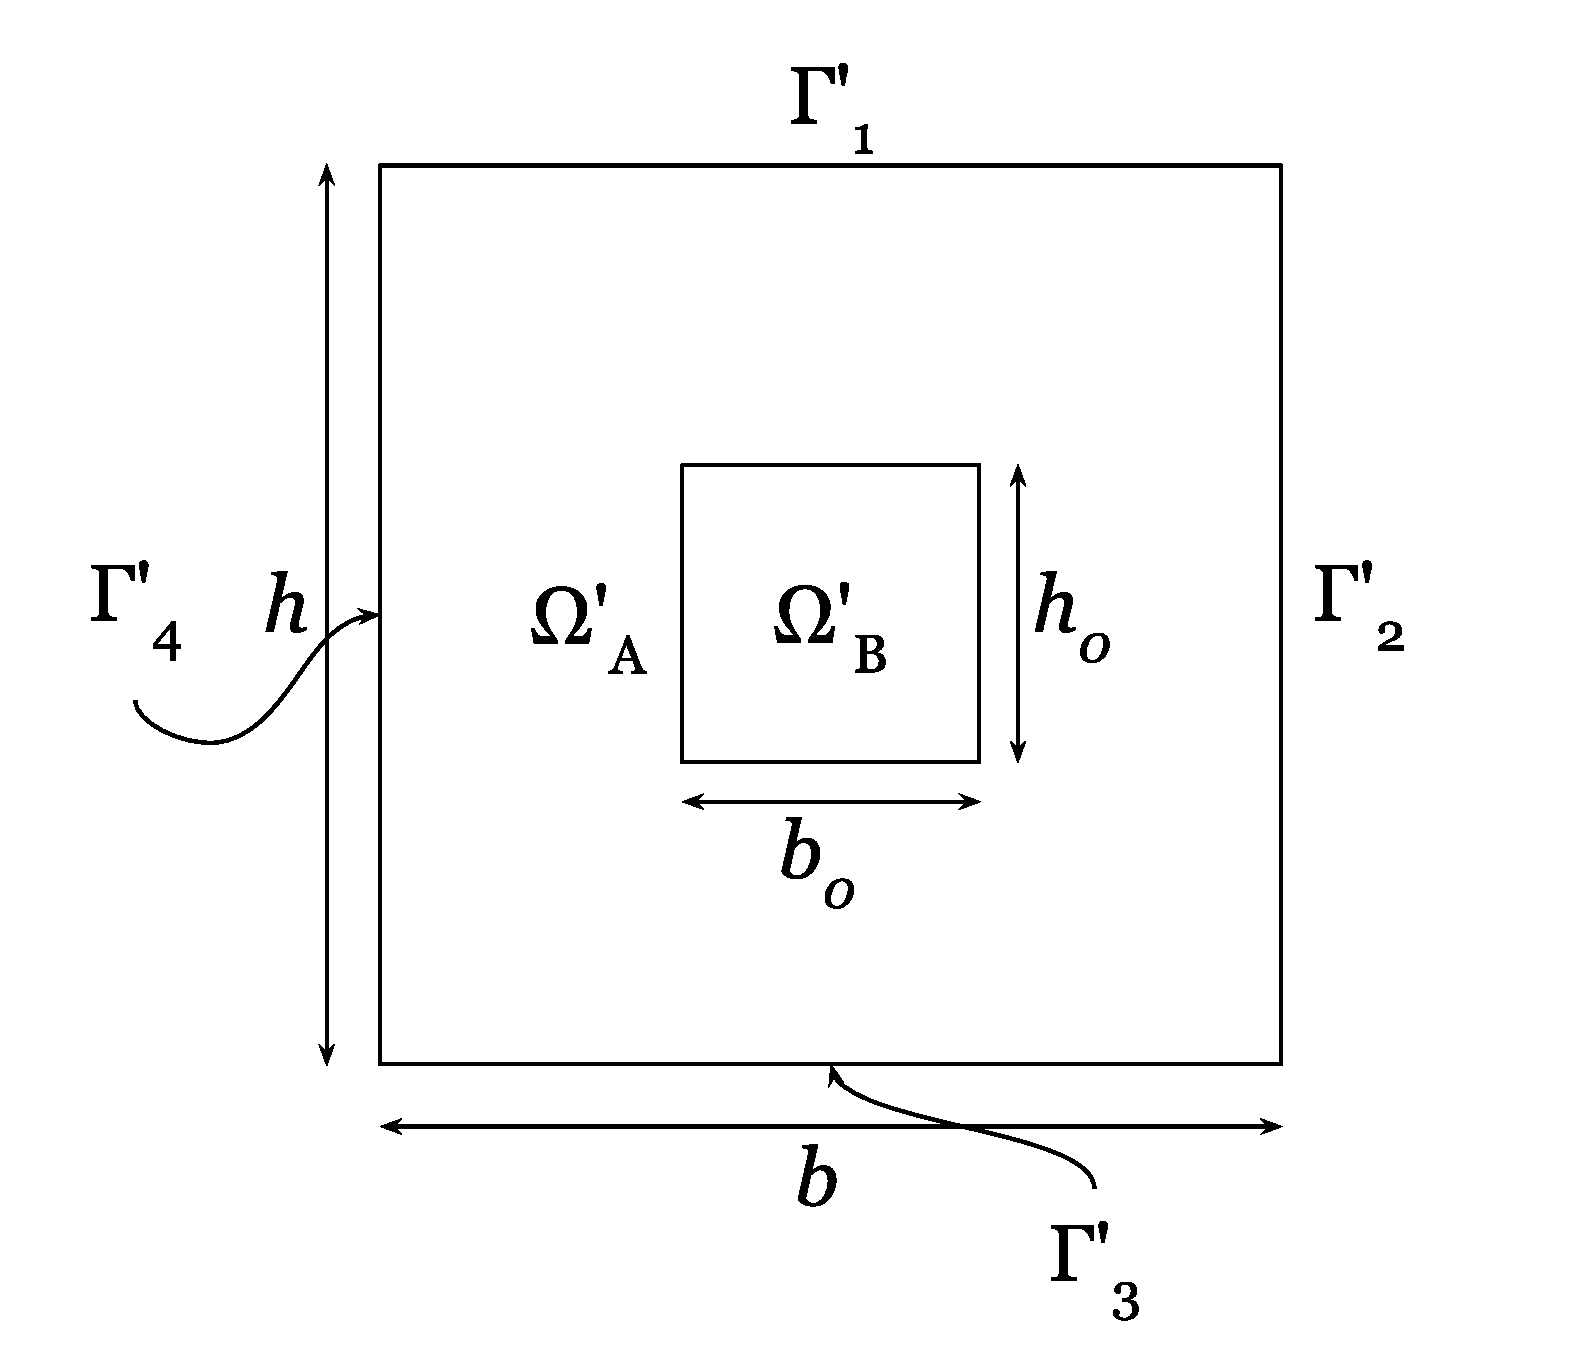
\includegraphics[width=0.7\linewidth]{domain.eps}
 \captionof{figure}{Considered domain $\Omega\prime$, with boundary $\Gamma$.}\label{fig:domain}
\end{Figure}The domain $\Omega_A$ has two Dirichlet boundary conditions, one Robin B.C. and one Neumann (natural) boundary condition: 
\begin{gather*}
\begin{align*}
    T|_{\Gamma_2\prime} &= T\arrowvert_{\Gamma_4\prime} = T_0,\\
    \left.\frac{\partial T}{\partial n}\right|_{\Gamma_3\prime} &= 0,\\
    K\left.\frac{\partial T}{\partial n}\right|_{\Gamma_1\prime} &= -\alpha \left(T_w - T_{\infty}\right).
\end{align*}
\end{gather*}